% LaTeX template for SIT723/SIT724 dissertation/exegesis for Deakin Honours and Masters students
% Authors:
% Dr. Chetan Arora, Academic Director (Coursework Research)
% Hon. A/Prof. Jacob L. Cybulski

\documentclass[oneside,12pt]{article}
\pagestyle{plain}

%%%-----PACKAGES------------------
%\usepackage[english,activeacute]{babel}
\usepackage[british,UKenglish,USenglish,american]{babel}
%\usepackage[utf8]{inputenc}

\usepackage{amssymb}
\usepackage[leqno]{amsmath}
\usepackage{amsfonts}
\usepackage{amsopn}
\usepackage{amstext}
\usepackage{amsthm}
\usepackage[textsize=small]{todonotes}
%\usepackage[disable]{todonotes}
\setuptodonotes{color=blue!30}
\usepackage{enumitem}
\usepackage{xy}

\usepackage{tikz}
\usetikzlibrary{cd}

\usepackage{verbatim}
\usepackage[colorlinks, backref, citecolor=blue]{hyperref}
\usepackage[numbers]{natbib}
\usepackage{makeidx}

\newcommand{\define}[2]{{\em #1}\index{#2}}


% Packages for special symbols and ornaments:
\usepackage{calrsfs}
\usepackage{fourier-orns}
%\usepackage{hieroglf} \newcommand{\hiero}{\textpmhg}
\usepackage{clock} %\ClockFrametrue\ClockStyle2
\usepackage[alpine, weather]{ifsym}
\usepackage{tabularx} % extra features for tabular environment
\usepackage{graphicx} % takes care of graphic including machinery
\usepackage{blindtext}
\usepackage{soul}
\usepackage{physics}
\usepackage{qcircuit}
\usepackage{subcaption} 
\usepackage{framed} 
\usepackage{authblk}

% Resolve rho and varrho symbols
\usepackage{mathptmx}
\DeclareSymbolFont{newfont}{OML}{cmm}{m}{it}% Computer Modern math font
\DeclareMathSymbol{\Epsilon}{3}{newfont}{15}% Symbol 15
\DeclareMathSymbol{\Rho}{\mathalpha}{operators}{"50}

% Formatting page
\usepackage{setspace}

% Notes in margins and switching them on and off (if needed)
\newcommand{\almarginpar}[1]{\leavevmode\marginpar[\raggedleft\small\textit{#1}]{}}
%\newcommand{\almarginpar}[1]{}

\providecommand{\ar}{\arrow}
\newcommand{\Em}{\mathbb M}


\frenchspacing

\providecommand{\cal}{\mathcal}
\renewcommand{\Bbb}{\mathbb}
\renewcommand{\frak}{\mathfrak}
\newenvironment{pf}{\begin{proof}}{\end{proof}}

%%%%%%%%%%%%%%%%%%%%
% Standard commands
%%%%%%%%%%%%%%%%%%%%

%%%%%%%%%%%%%%%%%%%%
% Calligraphic and bold letters. 
%%%%%%%%%%%%%%%%%%%%
\newcommand{\Aa}{{\Bbb{A}}}
\newcommand{\Aaa}{{\cal{A}}}
\newcommand{\Bee}{{\cal{B}}}
\newcommand{\Cee}{{\cal{C}}}
\newcommand{\Dee}{{\cal{D}}}
\newcommand{\Ef}{{\cal{F}}}
\newcommand{\Gee}{{\cal{G}}}
\newcommand{\Haa}{{\cal{H}}}
\newcommand{\Ai}{\cal{I}}
\newcommand{\Kay}{{\cal{K}}}
\newcommand{\El}{{\cal{L}}}
\newcommand{\Pee}{{\cal{P}}}
\newcommand{\See}{{\cal{S}}}
\newcommand{\Tau}{{\cal{T}}}
\newcommand{\Yu}{{\cal{U}}}
\newcommand{\Vee}{{\cal{V}}}
\newcommand{\Wu}{{\cal{W}}}
\newcommand{\Zee}{{\Bbb{Z}}}
\newcommand{\Emm}{{\frak{M}}}
\newcommand{\Be}{{\Bbb{B}}}
\newcommand{\Nat}{{\Bbb{N}}}
\newcommand{\Z}{{\mathbb Z}} % The integers
\newcommand{\Qyu}{{\Bbb{Q}}}
\newcommand{\Err}{{\Bbb{R}}}


%%%%%%%%%%%%%%%%%%%%
% Shortcuts for some Greek letters. 
%%%%%%%%%%%%%%%%%%%%
\newcommand{\lam}{{\lambda}}
\newcommand{\al}{\alpha}
\newcommand{\Gam}{\Gamma}
\newcommand{\alG}{\al\in\Gamma}
\newcommand{\sig}{\sigma}
\newcommand{\eps}{\varepsilon}
\renewcommand{\phi}{\varphi}
\renewcommand{\rho}{\varrho}

%%%%%%%%%%%%%%%%%%%%
% Basic commands. 
%%%%%%%%%%%%%%%%%%%%
\newcommand{\rest}{\restriction}
\newcommand{\unii}{\mathbb I}
\newcommand{\ntr}{{n\in\omega}}
\newcommand{\Ntr}{n\in{\Bbb{N}}}
\newcommand{\loe}{\leq}
\newcommand{\goe}{\geq}
\newcommand{\notloe}{\nleq}
\newcommand{\notgoe}{\ngeq}
\newcommand{\subs}{\subseteq}
\newcommand{\sups}{\supseteq}
\newcommand{\nnempty}{\ne\emptyset}
\newcommand{\argum}{\:\cdot\:}
\newcommand{\ovr}{\overline}
\renewcommand{\iff}{\Longleftrightarrow}

%%%%%%%%%%%%%%%%%%%%
% Topology. 
%%%%%%%%%%%%%%%%%%%%
\newcommand{\Cl}[1]{\overline{#1}}
\newcommand{\cl}{\operatorname{cl}}
\newcommand{\Int}{\operatorname{int}}
\newcommand{\w}{\operatorname{w}}
\newcommand{\dens}{\operatorname{dens}}
\newcommand{\eXp}{\operatorname{exp}}
\newcommand{\diam}{\operatorname{diam}}
\newcommand{\dist}{\operatorname{dist}}
\newcommand{\nbd}{\operatorname{nbd}}


%%%%%%%%%%%%%%%%%%%%
% Convexity. 
%%%%%%%%%%%%%%%%%%%%
\newcommand{\conv}{\operatorname{conv}}
\newcommand{\co}{\operatorname{co}}
\newcommand{\clco}{\operatorname{clco}}
\newcommand{\m}{\operatorname{m}}
\newcommand{\med}{\operatorname{med}}

\newcommand{\G}{{\mathbb G}}

%%%%%%%%%%%%%%%%%%%%
% Miscellaneous. 
%%%%%%%%%%%%%%%%%%%%
\newcommand{\id}[1]{{\operatorname{i\!d}_{#1}}} % identity morphism
\newcommand{\cf}{\operatorname{cf}}
\newcommand{\dom}{\operatorname{dom}}
\newcommand{\cod}{\operatorname{cod}}
\newcommand{\Dom}{\operatorname{Dom}}
\newcommand{\rng}{\operatorname{rng}}
\newcommand{\suppt}{\operatorname{suppt}}
\newcommand{\defi}{\stackrel{\rm df}=}
\newcommand{\pr}{\operatorname{pr}}
\newcommand{\liminv}{\varprojlim}

\newcommand{\symd}{\div} % <--- Symmetrical difference

\newcommand{\oraz}{\qquad\text{and}\qquad}

\setcounter{secnumdepth}{5}
\setcounter{tocdepth}{5}
\newcommand\subsubsubsection{\@startsection{paragraph}{4}{\z@}{-2.5ex\@plus -1ex \@minus -.25ex}{1.25ex \@plus .25ex}{\normalfont\normalsize\bfseries}}
\newcommand\subsubsubsubsection{\@startsection{subparagraph}{5}{\z@}{-2.5ex\@plus -1ex \@minus -.25ex}{1.25ex \@plus .25ex}{\normalfont\normalsize\bfseries}}

%%%%%%%%%%%%%%%%%%%%
% Some forcing commands. 
%%%%%%%%%%%%%%%%%%%%
\newcommand{\proves}{\vdash}
\newcommand{\forces}{\Vdash}
\newcommand{\Con}{\operatorname{Con}}
\newcommand{\Card}{{\frak{Card}}}
\newcommand{\Func}{\operatorname{Func}}
\newcommand{\poset}{{\Bbb{P}}}
\newcommand{\Forall}{\forall\;}
\newcommand{\Exists}{\exists\;}
\newcommand{\h}{\widehat}
\newcommand{\val}{\operatorname{val}}
\newcommand{\comp}{\parallel}
\newcommand{\incomp}{\perp}
\newcommand{\Es}{{\cal{S}}}
\newcommand{\meet}{\wedge}
\newcommand{\Meet}{\prod}
\newcommand{\join}{\vee}
\renewcommand{\Join}{\sum}
\newcommand{\Land}{\;\&\;}


%%%%%%%%%%%%%%%%%%%%
% Trees. 
%%%%%%%%%%%%%%%%%%%%
\newcommand{\Lev}{\operatorname{Lev}}
\newcommand{\lev}[2]{{\ell_{#1}#2}}
\newcommand{\Ht}{\operatorname{ht}}
\newcommand{\length}{\operatorname{length}}
\newcommand{\bd}{\partial}

\newcommand{\concat}{{}^\smallfrown}
\newcommand{\Reg}{{\frak{Reg}}}
\newcommand{\Ord}{{\frak{Ord}}}
\newcommand{\by}[1]{/_{#1}}
\newcommand{\club}{\operatorname{club}}
\newcommand{\proj}{\operatorname{proj}}
\newcommand{\otp}{\operatorname{otp}}
\newcommand{\Fin}{\operatorname{fin}}

%%%%%%%%%%%%%%%%%%%%
% Theorems and Propositions. 
%%%%%%%%%%%%%%%%%%%%
\newtheorem{tw}{Theorem}[section]
\newtheorem{wn}[tw]{Corollary}
\newtheorem{lm}[tw]{Lemma}
\newtheorem{prop}[tw]{Proposition}
\newtheorem{claim}[tw]{Claim}
\theoremstyle{definition}
\newtheorem{df}[tw]{Definition}
\newtheorem{ex}[tw]{Example}
\newtheorem{pyt}[tw]{Question}
\newtheorem{question}[tw]{Question}
\theoremstyle{remark}
\newtheorem{uwgi}{Remark}
\renewcommand{\theuwgi}{}

%%%%%%%%%%%%%%
% Create notes
%%%%%%%%%%%%%%
\usepackage{enumitem,amssymb}
\newlist{todolist}{itemize}{2}
\setlist[todolist]{label=$\square$}
\usepackage{pifont}
\newcommand{\cmark}{\ding{51}}%
\newcommand{\xmark}{\ding{55}}%
\newcommand{\done}{\rlap{$\square$}{\raisebox{2pt}{\large\hspace{1pt}\cmark}}%
\hspace{-2.5pt}}
\newcommand{\wontfix}{\rlap{$\square$}{\large\hspace{1pt}\xmark}}

% Cantor's stuff:
\newcommand{\Cantor}{2^\omega}

\hypersetup{
	colorlinks=true,       % false: boxed links; true: colored links
	linkcolor=blue,        % color of internal links
	citecolor=blue,        % color of links to bibliography
	filecolor=magenta,     % color of file links
	urlcolor=blue         
}

%%%-----ORIGINALLY SUGGESTED PACKAGES------------------
\usepackage{graphicx}
\usepackage{fontspec}
% \usepackage[utf8]{inputenc}
\usepackage{geometry}
\geometry{a4paper, inner=50mm, outer=20mm, left=48mm,  top=22mm, bottom=22mm, right=22mm, marginparwidth=40mm} %, showframe}
\usepackage{setspace}
\usepackage[document]{ragged2e}
% \usepackage{times,fullpage} 
% \usepackage{hyperref}
\usepackage{array}
\usepackage{wrapfig}
\usepackage{fancyhdr}
\usepackage{colortbl}
\usepackage{xcolor}
\renewcommand{\familydefault}{\sfdefault}
\hyphenpenalty=10000
\tolerance=10000
\graphicspath{ {Figures/}} %% Path to your Figure folder

%%% IF you need headers and footers
% \usepackage{fancyhdr}
% \pagestyle{fancy}
% \fancyhf{}
% \fancyhead[L]{\rightmark}
% \rfoot{\thepage}
% \renewcommand{\headrulewidth}{0pt}

%-------------DOCUMENT BEGIN-------------------
\begin{document}
\onehalfspacing
%========= Title Page
\thispagestyle{empty} 
\begin{titlepage}
    
\includegraphics[width=0.25\textwidth]{Deakin_Logo.jpeg}
    \begin{center}
       \vspace*{4cm}
       {\LARGE Quantum Computing in Radar Signal Analysis}
       \vspace{3cm}
    \begin{large}   
    
        {\bf Submitted as Research Report / Honours / Master Dissertation in SIT723}\todo{What would be the correct wording here?}
       \vspace{1cm}
        
        {\bf SUBMISSION DATE} \\
        T1-2022
        
       \vspace{3cm}
       \textbf{Mark Blashki}\\
       STUDENT ID 220228182 \\
       COURSE - Bachelor of Information Technology (Honours)
       \vfill

       {\bf \normalsize Supervised by: Hon. A/Prof. Jacob L. Cybulski }\\ \todo{Jacob - please confirm name and title}
       
    \end{large}  
   \end{center}
\end{titlepage}

%PAGE SETUP
% \textheight=22cm
% \textwidth=15cm
% %\hoffset=-1cm
% \hoffset=2.5cm
% \voffset=-2cm
% %\parindent=16pt
\setlength{\marginparwidth}{4cm}
\reversemarginpar

%-----------Abstract----------
\newpage 
\thispagestyle{plain} 
\pagenumbering{roman}
\section*{Abstract}

This report explores the potential application of quantum computing methods in radar signal analysis for \ac{EW}.
With traditional signal processing techniques nearing the edge of classical computing's extent, new approaches are required to keep up with emerging threats.
Much research has been conducted on quantum computing and it's potential applications to signal processing, however, little work has been done in its application to radar signal processing for \ac{EW}.
This report presents a survey of the current state of research, as well as an exploratory probe into how quantum methods can encode, detect, and characterise radar signals.
Novel quantum methods for encoding signals, determining radar pulse boundaries, and frequency characterisation will be presented.\todojc{I think your abstract should end here, the rest is for the introduction}
The milestones for the project are:
\begin{enumerate}
    \item Acquire a signal simulator; generate source data with valid radar models
    \item Identify, and implement several quantum-based encoding methods that convert sampled time-domain radar signals into a form which prepares them for further quantum processing.
    \item Develop a method for quantum-based pulse detection of a radar signals. Test the method by varying the type and quality of radar signals. Present quantifiably measurable results.
    \item Determine a quantum method for estimating a radar signal’s frequency. Test the algorithm on a variety of radar signals and present quantitative results of its performance.
\end{enumerate}

The research plan is, in the first phase in T1, to conduct experiment 1 - encoding. In the second phase - T2, to continue with executing experiments 2 and 3.

%---------Table of Content, Figures and Tables--------
\newpage
\begin{singlespacing}
\tableofcontents
\end{singlespacing}
\setlength{\parskip}{1em}
\renewcommand{\baselinestretch}{2.0}

\newpage
\listoffigures
\listoftables

% Main body of Thesis
%========= Start of Thesis 
\newpage 
\pagenumbering{arabic}
\setcounter{page}{1}
\onehalfspacing

%%-------SECTIONS
%%------ Include files for each section
%========= Introduction
\section{Introduction}
\label{sec:introduction}

In the complex and ever-evolving world of \ac{EW}, quantum computing could provide the ability to understand radar signals in novel ways, never before seen in this field. 
It is widely recognised in the discipline of electronic warfare that traditional signal analysis techniques are still bounded by computational constraints, so in order to maintain strategic advantage, new techniques are continuously needed in order to keep pace with emerging threats. 
Quantum computing may promise a paradigmatic shift in extracting actionable insights from massive and complex \ac{EW} datasets. 

Recent research has demonstrated a great potential for quantum computing to address the challenges of modern signal processing
\cite{somma_quantum_2019, daskin_walk_2022},
however little work has been devoted to its applications in \ac{EW} signal processing, and more specifically radar signal processing 
Therefore, this report explores the question of how quantum technology may be applied
to radar signal processing in EW
At first, a survey of the current state of research will be conducted for radar signal analysis and quantum signal processing. 
Then, an empirical inquiry into the subject will be presented, aiming to determine 
how quantum methods can be used to encode, characterise, and de-interleave radar signals.
Finally, a discussion of results, examination of limitations, and consideration for future work will be provided. 
 
Despite quantum computing holding much promise, its potential in this field remains largely unexplored. This report will present a background and preliminary investigation into how quantum computing can be utilised in the dynamic landscape of electronic warfare. 

\subsection{Background}~\label{subsec:background}

Radar is "an electrical system that transmits \ac{RF} \ac{EM} waves toward a region of interest and receives and detects these EM waves when reflected
from objects in that region."\cite{richards_principles_2010}. The name radar originates from a portmanteau of \textit{Radio Detection and Ranging}\cite{the_joint_board_on_scientific_information_policy_radar_1945}, hinting at it's founding objectives in the defence context. In the modern day, radar is used in many civilian and military applications \cite{merrill_i_skolnik_radar_nodate, desai_how_2022}:
\begin{itemize}
    \item Aerospace - weather, navigation, approach, altitude, identification
    \item Maritime - navigation, collision avoidance,  
    \item Ground Penetrating - archaeology, mining, oceanographic sounding
    \item Space - spacecraft and celestial monitoring
    \item Automotive - civilian and law enforcement
    \item Industrial - fluid sensing, speed measurement
    \item Medical
    \item Atmospheric / Weather
    \item Electronic Warfare
\end{itemize}

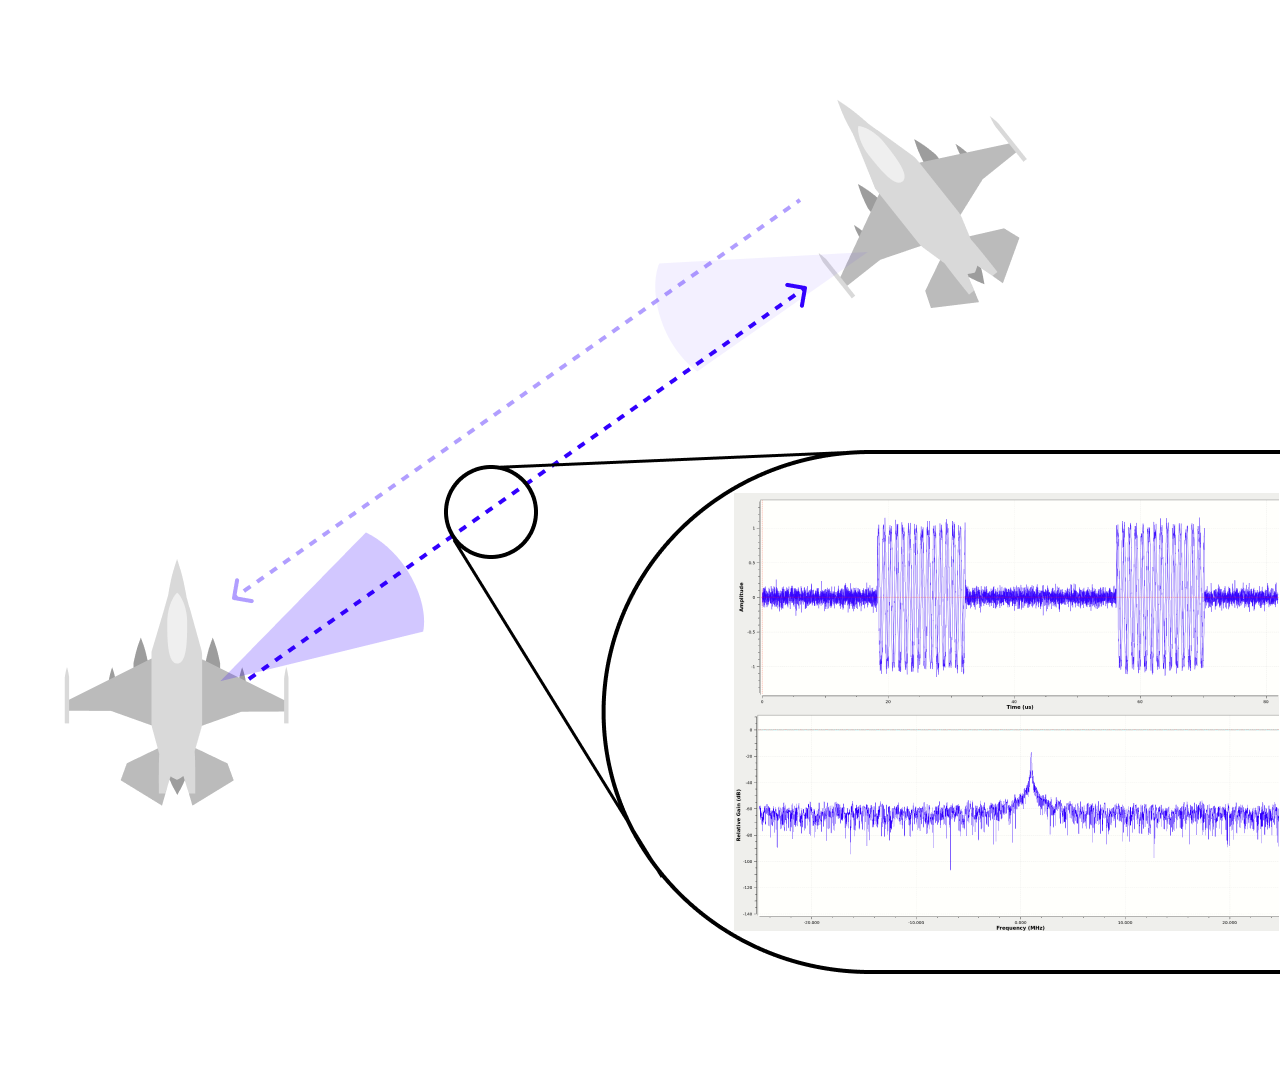
\includegraphics[width=\textwidth]{Figures/Senario_ Single Radar; single signal.png}

Since radar systems were invented in 1930 \cite{degering_invention_2018}, their usage has become increasingly widespread. As a result, the electromagnetic environment has become densely populated, with a multitude of different emitters posing a challenge of unintentional interference with operating radars \cite{degering_invention_2018}. However, their widespread adoption - particularly in the defence context - yields the potential to identify the location and type of emitters in the area of operation.\todo{Passive; ESM}
This subject has been encompassed in the broader discipline of \ac{EW}. \ac{EW} is defined by David Adamy \cite{adamy_13_2001} as "the art and science of preserving the use of the electromagnetic spectrum for friendly use while denying its use to the enemy"\todo{I think a different definition would be best here, or perhaps referencing ELINT...}.

\ac{ESM}, a sub-field of \ac{EW}, where \ac{ESM} as "the receiving part of EW"\cite{adamy_13_2001}, of which radar is the principal element".

\todo{Describe the importance of radar \ac{ESM} here. Who cares and why? }

\todo{Principles of radar}

A typical radar system is made up of at least one of each: radio transmitter, radio receiver, antenna, and display \cite{stimson_introduction_1998}. % There was a more precise definition somewhere with a 'signal processor' element.

% The ESM pipeline
% IQ Data -> Pulse Detection -> Pulse Compression -> Doppler Processing -> Constant False Alarm Rate (CFAR) Detection -> Target Association -> Tracking -> Classification -> Decision

% ------------
% BELOW IS A GENERAL OUTLINE. It highlights the sequence of radar processing.
% ------------
% Pulse Detection:
% - Matched filtering or other pulse detection algorithm to identify radar pulses
% - Thresholding to remove noise and false detections

% Pulse Compression:
% - Matched filtering or other pulse compression algorithm to enhance SNR of pulses
% - Windowing to reduce sidelobes and improve spectral properties

% Doppler Processing:
% - Fourier transform or other Doppler processing algorithm to estimate target velocity
% - Doppler filtering to reject clutter and interference

% CFAR Detection:
% - CFAR algorithm to detect targets in the presence of noise and clutter
% - Adaptive thresholding to adjust detection threshold based on local noise level

% Target Association:
% - Clustering or other target association algorithm to group detections into tracks
% - Filtering or smoothing to reduce track jitter and improve accuracy

% Tracking:
% - Kalman filter or other tracking algorithm to predict target state and estimate measurement errors
% - Maneuver detection and tracking to handle agile targets

% Classification:
% - Feature extraction and classification algorithm to identify target type
% - Machine learning or rule-based classification

% Decision:
% - Target prioritization and threat assessment
% - Decision making based on mission objectives and rules of engagement
% - Display and dissemination of results
% ------------------------------

\todo{Link back to:\ac{ESM} \ac{ECM} \ac{ECCM}. Here, consider providing a precise definition of \ac{ESM}. Also, somewhere here, a mention of \ac{ELINT} should be made}

For the radar to achieve its objectives, it must be able to convert observed data into actionable information, thereby requiring some degree of information processing. Herein lies the general challenges in \ac{ESM} - the detection, location, and identification of targets, which will now be explored. % Cite 'detection, location and identification' - I think the precise term is 'analysis'.

First, however, a conceptual schematisation of this system must be made in in terms of its inputs, process, and outputs. In \ac{ESM}, inputs consist of EM fluctuations that vary over time. They are almost always received by an antenna (or antennas) which may be subsequently manipulated in the analogue and digital domains. These fluctuations, henceforth \textit{signals} (not to be confused with communications signals), are the essential information carriers in the signal processing operation. There also exist inputs derived from the nature of the radar system configuration itself. These may include the antenna configuration and receiver architecture which will not here be considered, but is noted by the author as being of significant relevance to kinematic measurement and capability constraints.

Since the signals of interest are those emitted by radar systems, the received signals exhibit phenomenal qualities corresponding to those of the originating radar, namely: \cite{avionics_department_electronic_2013} 5-8.1
\begin{itemize}
    \item Frequency (\ac{RF}): Intrapulse frequency, modulation (and associated modulation parameters); Interpulse: phase coherence.
    \item Amplitude (power)
    \item \ac{DOA} / \ac{AOA}
    \item \ac{TOA}
    \item \ac{PRI}, \ac{PRF}
    \item \ac{PRI} type
    \item \ac{PW}
    \item Scan type and rate
    \item Lobe duration (beam width or dwell)
\end{itemize}

The role of the processing step, is to convert the 'raw' signal into these parameters. Optimally, the parameters equal those nominally transmitted by the target radar.
These are generally extracted from the incident \ac{EM} signals and may be treated independently as outputs themselves. Typically, however, further analysis may be may conducted to yield very granular information. Information that \ac{ESM} seeks to understand addresses many facets:
\begin{itemize}
    \item Detection
    \item Target characteristics \cite{jenn_radar_2007}
    \begin{itemize}
        \item target size - return amplitude
        \item target shape - from discrete scan returns
        \item target material composition
        \item moving parts (modulation of the return)
    \end{itemize}
    \item Target identification
    \item Kinematic parameters and tracking(range, direction, speed, \ac{AOA})
\end{itemize}

\todo{Introduce multi-radar concept. }
\todo{Illustrate a scenario to make the problem more evident.}

\subsubsection{Research Question}
% To what extent can quantum computing methods can quantum computing be used to understand radar signals?
How can quantum computing methods be used to in an ESM function to detect the types and characteristics of radar signals in the defence context?

\subsubsection{Research Objectives}
\begin{itemize}
    \item Acquire a source data emulator to be used to test and verify quantum implementations.
    \item Identify the specific types of radar signals used in radar systems and their key signal parameters, based on an analysis of publicly available technical documents and datasets.
    \item Develop a quantum-based encoding method that converts sampled time-domain radar signals into qubits.
    \item Validate the quantum encoding method by evaluating the expressivity, complexity, and qualitative suitability.
    \item Develop a method for quantum-based pulse detection of a radar signals that vary in type and quality. The method must be quantifiably measurable.
    \item Validate the quantum pulse detection method by evaluating the accuracy of pulse boundary detection and signal-to-noise tolerance.
    \item Determine a quantum method for estimating a radar signal's frequency.
    \item Validate the frequency estimation method by evaluating the accuracy and signal-to-noise tolerance.
\end{itemize}

\subsection{Scope}

\subsubsection{Out of Scope}

\todojc{This section may need some initial statement and each bullet point some brief explanation}\begin{itemize}
    \item Hardware
        No consideration of hardware constraints 
    \item Anything down-stream of identification of radar signals. (e.g., display, databasing, data fusion, etc.)
    \item \ac{SAR} and antenna-specific computation (i.e., bistatic/multistatic antenna setups)
    \item Imaging
    \item Kinetic estimation (range, velocity, angle of arrival, etc.)
    \item Forecasting
    \item Active emission.
    \item Simulation / emulation
    \item Radio signals only; sub-millimetre-wave technology is not considered.
    \item Resource allocation
    \item Ambiguity analysis
    \item Tracking
    \item Multipath effects
\end{itemize}

% Identify the challenge with multi-radar environments.

% Provide a brief outline of the genus of classical processing approaches.\
% Introduce quantum computing, and provide an abstracted overview of its potential application to this field.
% Conclude the case for quantum computing in ESM. Providce an implicit definition of the research question
% Identify the challenges with quantum computing.

\begin{quote}
    \textit{"The increased pulse density created by the deployment of pulse Doppler radar, both enemy and friendly, has created demand for systems with a high signal processing capability"} \cite{pettersson_illustrated_1992} p. 42
\end{quote}


% ---------------
% OLD EXPLANATION
% ---------------
% One category of radar is pulsed-Doppler which emits energy in high-frequency pulses. The characteristics of the pulses impact the range resolution, with shorter pulses allowing for higher resolution because the receive signal is too shorter. However, the trade-off is that a shorter pulse means less time for the emission to illuminate the target, and therefore less return amplitude and shorter maximum range. One way to counter this issue is to use a technique named ‘pulse compression’. In principle, the technique bypasses this limitation by transmitting infinitely short pulses. How? By means of frequency modulation; by ramping the transmission frequency linearly up or down. The difficulty is: how to receive a single pulse over these many frequencies. The solution is in using an analogue filter with a non-linear phase response which causes lower frequencies to be ‘delayed’ or phase-shifted, more than higher frequencies, In effect it ‘compresses’ the returned pulse into a higher power pulse, thereby increasing both range resolution, and maximum range. This, however, is not enough. Higher range and resolution are desired – and that means more power! A single pulse is alone insufficient in solving the problem; the solution lays in multiple pulses. By sending more than one pulse, one increases the average transmitted power on the target (and thus returns). With multiple pulses, the chances of a return being intercepted are increased. These pulses must be transmitted consecutively therefore, at some Pulse Repetition Frequency (PRF). However effective upon first thought, a limitation always arises – range ambiguity. If a pulse is transmitted and, before the its return received, another pulse arrives,  \cite{parker_chapter_2010}

% --------------
% OLD OBJECTIVES
% --------------
% In the processing functional block, the problems for radar are, in sequential order:
% \begin{itemize}
%     \item How to distinguish between the different categories of signals: communications, interference, radar, and noise.
%     \item Then, after having understood what signals are radar intercepts, identifying which belong to the same originating receiver. 
%     \item Once, a radar signal has been de-interleaved, how to identify the originating emitter, given some a priori understanding of the operational environment.
% \end{itemize}
% \begin{itemize}
%     \item To further understand the principles of operation of passive radar systems, including their ability to detect and identify emitters in complex electromagnetic environments.
%     \item To critically evaluate existing literature on radar systems and quantum computing to effecively communicate existing the academic knowledge, and to show a capability to conduct independent future research.
%     \item To identify the possibilities of using Quantum Computing in Radar signal analysis; to also identify three candidate avenues; to explore one in enough depth to evaluate potential feasability though the creation of a technical solution
%     \item To prioritize research topics based on their level of desirability and feasibility, and to develop a plan for executing research projects within a defined timeline and scope.
%     \item To communicate research findings effectively to a technical audience.
% \end{itemize}
% \begin{itemize}
%     \item Identify a candidate method, or methods for converting continuously varying parameterised radar signals into into discrete radar modes using quantum methods?
%     \item Is it possible, and to what extent are quantum methods effective in de-interleaving and signal clustering?
%     \item Can quantum computing effectively track a radar signal intercept, and how well?
%     \item %\almarginpar{Would the last two-four be in too hard basket for the time frame? May be better to leave those for the motivation section - if we could do the previous then we'd be able to do the following?}
%     In the radar context, can, and how well are quantum computing methods disposed to help in reducing noise, interference, and clutter?
% \end{itemize}

\section{Literature Review}~\label{sec:literature}

% 1. Academic references - explain / summarise them\\
% 2. Develop a meta-model of their fundamental argument, challenges, deficiencies, and strengths\\
% 3. Compare their differences, similarities, and whether or not they agree. (If they all agree, more sources should be found); how they interrelate.\\
% 4. Next, the exposition of the problem space (radar signal analysis) should be written, being lean enough so as to only explain the content of the referenced academic sources. I.e., the challenges faced should be fully developed.\\
% 5. Following which, a more precise formulation of problems should be undertaken.

%-------- Objectives of Honours
\subsection{Course Objectives}

%-------- Scope
\subsection{Scope}

Depending on the speed of progress throughout the honours project, the scope of the project will change. The extent of exploration into these concepts is wholly dependent on the available time. The scope should therefore not be defined fixed in time, but rather prioritised by level of desirability. At each level of scope, a definition of done must have been both defined and then met before proceeding to the next.

\begin{enumerate}
    \item 
\end{enumerate}

%-------- Use Cases / context
\subsection{Use Cases of Radar / contexts}

\begin{itemize}
    \item 3-5 Functional categories and uses of Radar: \cite{}
    \begin{itemize}
        \item Aerospace - weather, navigation, approach, altitude, identification
        \item Maritime - navigation, collision avoidance,  
        \item Ground Penetrating - archaeology, mining, oceanographic sounding
        \item Space - craft and celestial
        \item Automotive - civilian and law enforcement
        \item Industrial - fluid sensing, speed measurement
        \item Medical - tomography etc
        \item Atmospheric / Weather
        \item Defence / Electronic Warfare
   \end{itemize}
\end{itemize}
%
%-------- Objectives
\subsection{Objectives of Radar}

The original object of radar lay in the name itself: a portmanteau of \textit{Radio Detection and Ranging}. \cite{policy_radar_1945}

Today, the desired outputs of Radar systems are:

\begin{itemize}
    \item range
    \item velocity
    \item DOA (az/el)
    \item TOA
\end{itemize}

In addition to radar signature / scattering cancellation:
% TODO: figure out how to cite stuff. Following list derived from p4 of https://faculty.nps.edu/jenn/seminars/radarfundamentals.pdf
\begin{itemize}
    \item target size - return amplitude
    \item target shape - from discrete scan returns
    \item target material composition
    \item moving parts (modulation of the return)
\end{itemize}

% Also these functions
% \begin{itemize}
%     \item Detection
%     \item tracking
%     \item Identification
%     \item Range
%     \item Direction
%     \item Speed
%     \item Imaging
%     \item Navigation
% \end{itemize}

%-------- Shall a history be applicable here? i.e., a chronological development of the technology of radar

%-------- Principle of Operation
\subsection{Radar: Principles of Operation}

\subsubsection{Option 1}

The primary interest of this option is in passive radar, i.e., radars which generally do not transmit energy and listen to a return.

One functional mode of radar is a search mode: where the system’s objective is to interrogate the electromagnetic environment to detect and identify emitters. The only information that radars are given is the signals which it receives, and its location in space and time (as well as some prior understanding of the operational environment). Due to the nature of the operating context, modern radars may receive many incident signals in a short period of time. Within such received signals, there may exists a number of constituent parts: communications signals, radar signals, interference (whether intentional or not), and noise (being environmental, or system). For signals originating from radars, they vary in several dimensions: see radar domains. Noise is generally constant, but limits the receiver’s ability to detect a given signal’s presence. Interference is any signal which interferes with the receiver’s ability to perform its function – either fully or partially. The functional operation of the receiver is: signal input (coming from antenna), RF front-end, digitisation, and processing. In each stage, the signal may change characteristics and formats based on a variety of filtering and processing operations.

In the processing functional block, the problems for radar are, in sequential order:

\begin{itemize}
    \item How to distinguish between the different categories of signals: communications, interference, radar, and noise.
    \item Then, after having understood what signals are radar intercepts, identifying which belong to the same originating receiver. 
    \item Once, a radar signal has been de-interleaved, how to identify the originating emitter, given some a priori understanding of the operational environment.
\end{itemize}

In each of these phases, there are two other activities which may take place:

\begin{itemize}
    \item Display for use by an operator
    \item Tracking – identifying the Direction of Arrival (DOA) and rate of change of DOA, to track a target. Tracking may be undertaken at the same time as the search mode – named search-and-track.
    \item In search-and-track modes, there exists a problem in how to allocate dwell time to each target track, versus in searching some area.
\end{itemize}

\subsubsection{Option 2}

The primary interest of this option is in active radar, i.e., radars which emit energy and listen to a return.

One category of radar is pulsed-Doppler which emits energy in high-frequency pulses. The characteristics of the pulses impact the range resolution, with shorter pulses allowing for higher resolution because the receive signal is too shorter. However, the trade-off is that a shorter pulse means less time for the emission to illuminate the target, and therefore less return amplitude and shorter maximum range. One way to counter this issue is to use a technique named ‘pulse compression’. In principle, the technique bypasses this limitation by transmitting infinitely short pulses. How? By means of frequency modulation; by ramping the transmission frequency linearly up or down. The difficulty is: how to receive a single pulse over these many frequencies. The solution is in using an analogue filter with a non-linear phase response which causes lower frequencies to be ‘delayed’ or phase-shifted, more than higher frequencies, In effect it ‘compresses’ the returned pulse into a higher power pulse, thereby increasing both range resolution, and maximum range. This, however, is not enough. Higher range and resolution are desired – and that means more power! A single pulse is alone insufficient in solving the problem; the solution lays in multiple pulses. By sending more than one pulse, one increases the average transmitted power on the target (and thus returns). With multiple pulses, the chances of a return being intercepted are increased. These pulses must be transmitted consecutively therefore, at some Pulse Repetition Frequency (PRF). However effective upon first thought, a limitation always arises – range ambiguity. If a pulse is transmitted and, before the its return received, another pulse arrives,  \cite{parker_chapter_2010}


%-------- Signal characteristics
\subsection{Characteristics of Radar Signals}

Domains: 
\begin{itemize}
    \item pulse params
    \item frequency
    \item PRF / PRI
    \item scan
    \item Modulation (and associated params)
    \item power
    \item polarisation
    \item PRF jitter / patterned PRF
    \item coherence
\end{itemize}

Pulse Descriptor words

%-------- Challenges

\subsection{Challenges in Radar signal analysis}

Here, note the areas in which overcoming challenges using classical computing is difficult or impractical.

\begin{itemize}
    \item Identification
    \item De-interleaving
    \item Imaging
    \item Clutter rejection
    \item LPI detection
    \item Noise reduction	
    \item Ambiguity analysis
    \item Parameter extraction
    \item Resource allocation
    \item Tracking
    \item Interference reduction
    \item Beamforming
\end{itemize}

%-------- Methods in achieveing challenges
\subsection{Methods}

%-------- Current challenges in those methods
\subsection{Open issues}

% Research question
\subsection{Research question}

Ideally, select 2-3 potential small, and well defined problems from which one may be selected for future formulation of a subsequent research inquiry.



% C. Wohlin, P. Runeson, M. H ̈ost, M. C. Ohlsson, B. Regnell, and A. Wessl ́en. Experimentation in Software Engineering. Springer Science & Business Media.
% M. Oivo, P. Kuvaja, P. Pulli, and J. Simil ̈a. Software engineering research strategy: Combining experimental and explorative research (eer). pages 302–317. Springer


\section{Research Design \& Methodology}~\label{sec:design}

In this section will be discussed the various research methods and techniques that will be used in this study.
First is the research methodology, wherein an examination of approaches will be made.
Secondly, the data environment will be defined, along with the controlled variables.
Finally the research design will be presented, followed by a discussion of the data collection methods, data analysis techniques, and methods for ensuring the validity the findings.

\todojc{The chapter should include two parts, i.e. the overall research methodology with justification (from the research question and objectives) and the details of your research design (what steps are to be taken as part of your research). The latter can be visualised as a chart of what are the research phases (which may include what would happen in T1 and then in T2) with the some description and justification. Most likely this would relate to your research objectives derived from your research question.}

%%% The methodological framework
\subsection{Research Methodology}
% RQ: (but different!)
This investigation aims to determine how can quantum computing methods be used to in an \ac{ESM} function to detect the types and characteristics of radar signals in the defence context.
% Partitio
Three aspects of this question will be explored: quantum encoding, pulse detection, and frequency estimation algorithms.
% Various research methodologies may be employed
Various research methodologies may be used to answer this question, including experimental, surveys, observational, and case study approaches.

% Experimental
\todojc{YOu need some refs for support here}Experimental research appears to be the most suitable methodology as it allows for well-defined set of inputs and dependents, that ultimately result in objective and precise data that can be analyzed statistically.
This enables a more indicative identification of the true nature of the quantum algorithms under test, thereby providing a deeper understanding of the solution itself.
In this respect, an experimental approach more truthfully validates the performance and consequent suitability of these new methods, thus increasing the reliability and generalisability of the results.
Furthermore, by systematically testing various scenarios, the experimental methodology attacks the problem from multiple aspects, thereby allowing for the discovery of new patterns and unexpected results - more than what could be achieved by any other of the alternative approaches. 

% Rebuttal
As there are few attempts at using quantum methods in radar signal processing, survey methodology, while useful for accumulating existing domain expertise (in the form of attitudes, beliefs, and opinions), cannot adequately and concretely examine the feasibility of such an unexplored approach to \ac{ESM}.
In other words, it is only by knowing a quantum algorithm that, through study, its nature can be understood.
Similarly, the scant availability of research on the topic, as revealed by the literature review, renders observational research methodology unsuitable.
Finally, unlike experimental approaches, a case study methodology is less generalisable and replicable.

% .: Experimental
For these reasons, the methodological framework adopted, for the three aspects of the research question, is experimental. 
% Describe basili
The approach adopted will be that of Basili et al. \cite{basili_experimentation_1985}.

% No hypothesis
Given little accessible research on the combination of quantum computing and \ac{ESM} signal analysis, this study will not present any \`{a} priori hypotheses, as there is not enough evidence to make a considered judgement.
% .: Exploratory
This is therefore an exploratory enquiry, intended to understand the feasibility of these quantum techniques and identify areas for further investigation, in contrast to the alternative confirmatory approach.
In this context, the framework adopted is like that of Olivo et al. \cite{oivo_software_2004}, wherein it is both experimental and exploratory.
It is also inductive, in the respect that the study will derive findings from data gathered during the research process rather than from an existing theoretical framework for quantum \ac{ESM} analysis.

\todojc{Nice tables but the reader will not understand what they mean - you need to discuss them in text - note that tables and figures do not speak for themselves - you need to help them!}According to the experimental framework, the \textit{definition} of the experiment is defined in Table \ref{tab:exp_definition}, \textit{planning} in Table \ref{tab:exp_planning}, and \textit{operation} in Table \ref{tab:exp_operation}.

Under Basili's methodology, the definition states the context and intent of the experiment.
In Table \ref{tab:exp_definition}, each experiment is described, taking particular note to the scope, which for experiment 1 is multi-project - as there are multiple algorithms being evaluated; and for experiments 2 and 3 being a single-project - as a single aretefact will be developed and evaluated.
The domain specifies the problem space the experiment intends to solve.


\begin{table}[ht]
\caption{Experimental definition}
\label{tab:exp_definition}
\begin{tabular}{p{0.16\linewidth}|p{0.28\linewidth}p{0.28\linewidth}p{0.28\linewidth}}
\hline
& Experiment 1: Quantum encoding & Experiment 2: Pulse detection & Experiment 3: frequency estimation \\
\hline
Motivation & To assess & To understand & To understand \\
Object & Pulsed-Doppler radar & \ac{CW} radar & \ac{FMCW} radar, pulsed \ac{CW} \\
Purpose & so that their performance and nature may be understood & so that pulses can be associated to individual radars & so that the frequency of a pulse can be extracted and used for further   analysis \\
Perspective & Researcher & Researcher & Researcher \\
Domain & Quantum encoding methods for ESM signals & Quantum pulse detection algorithm & Quantum frequency algorithm \\
Scope & Multi-project & Single project & Single project \\
\hline
\end{tabular}
\end{table}

Experimental planning is specified in Table \ref{tab:exp_planning}, where each run has defined the design, criteria, and measurement.
While more details are provided regarding the design of each experiment in \ref{sec:research_design}, the categories are: completely block, where the treatments (datasets), are applied to different blocks (encoding methods), whereas randomised block indicates that the treatments are applied to homogeneous groups (singular quantum algorithms).
The criteria is what is intended to be measured, while the measurement is the values which are being recorded.

\begin{table}[ht]
\caption{Experiment Planning}
\label{tab:exp_planning}
\begin{tabular}{p{0.16\linewidth}|p{0.28\linewidth}p{0.28\linewidth}p{0.28\linewidth}}
\hline
& Experiment 1: Quantum encoding & Experiment 2: Pulse detection & Experiment 3: frequency estimation \\
\hline
Design & Randomised block & Completely randomised & Completely randomised \\
Criteria & the quality and suitability of the method & An accurate  indication of pulse edge & An accurate frequency indication given some encoded signal input \\
Measurement & circuit size, expressibility, sampling capacity, bandwidth, and   computational efficiency & precision, recall, and F1 metrics & \ac{RMSE} frequency error, aggregated over all samples. \\
\hline
\end{tabular}
\end{table}

Experimental operation is defined in Table \ref{tab:exp_operation} with the quantum methods being all pilot studies and all using GNU radio.
The analysis of each method differs, but the encoding is analysed by a plot of the metrics (or \textit{measures}, as defined in Table \ref{tab:exp_planning}, for each encoding method.
Experiments 2 and 3 are presented using a variety of histograms, tables, and scatter plots.

\begin{table}[ht]
\caption{Experiment Operation}
\label{tab:exp_operation}
\begin{tabular}{p{0.16\linewidth}|p{0.28\linewidth}p{0.28\linewidth}p{0.28\linewidth}}
\hline
& Experiment 1: Quantum encoding & Experiment 2: Pulse detection & Experiment 3: frequency estimation \\
\hline
Preparation & Pilot study & Pilot study & Pilot study \\
Execution & Collection and validation Automated by GNU radio & Collection and validation Automated by GNU radio & Collection and validation Automated by GNU radio \\
Analysis & Plots of \textit{measure} (cf. Table \ref{tab:exp_planning}) vs encoding model &
\begin{itemize}
    \item data-table of metrics
    \item Histogram of measured pulse boundaries
    \item Scatter plot of measured vs actual pulse boundaries
\end{itemize}
&
\begin{itemize}
    \item data-table of metrics
    \item Histogram of measured results at different frequencies
    \item Scatter plot of measured vs actual frequency
\end{itemize}\\
\hline
\end{tabular}
\end{table}

\subsubsection{The data environment}

% Controlled and simulated
A choice of simulated conditions arose by necessity, since acquiring sample radar systems is impractical, cost prohibitive, and more importantly - out of scope.
It was therefore pertinent that a radar signal simulator be acquired.

%%% Experimental Partitio
To address each aspect of the research question - encoding, detection, and frequency estimation - a unique experimental design is required that takes into account the particular characteristics of the problem.
%%% General Criteria
In each case, the method's performance will be evaluated using quantitative measures.
As a whole, this research is to understand \textit{how} these methods may be used, but specifically not \textit{how well}.
The \textit{measures}, as defined in Table \ref{tab:exp_planning}, provide an indication as to the error rate (and thereby performance) of the quantum methods, however the quantum algorithms have quite fundamental differences in output when compared to classical methods, so its less meaningful to draw an explicit comparison between the two.
This study is therefore more of an enquiry into method, rather than a normative study of performance.

%%% Sample nature and collection
% Describe the nature sample (source data)
\todojc{All these seem very unorganised pieces of facts, which signal type if neeed where?}Each of the approaches perform different functions and therefore require different input data, but in general, the inputs are point source radar signals \cite{chakravorty_what_2018}.
Assumed to have been measured from the operating environment, these signals are simulated and sampled as input to each experiment.
Qualities of these signals are particular to the combination of source radars themselves, however in general, each sample is a complex number.
Complex data types are often employed in classical signal processing algorithms to capture phase and magnitude information of the radar signals, which are typically characterized by a sinusoidal nature.
For these reasons, the interface to the quantum implementations will be complex samples, varying in time.
The generated samples have a resolution of \(64\) bits: \(32\) bit wide floating point numbers for each real and imaginary coefficients.

% Data Collection - how is it collected?
To achieve the objective of acquiring radar signal test data a signal emulator - GNU Radio \cite{gnu_radio_contributors_gnu_2022} will be acquired and validated. 
The reason for using a signal simulator is due to its reproducibility, flexible scenarios, and wide access to the research community.
GNU radio specifically was chosen primarily on this basis, but also for its support of Python signal processing tools.

It has the capability of generating a set of radar signals exhibiting various degrees of signal quality and environmental situations. 
The variable signal quality refers to a signal-to-noise ratio, and environmental conditions refer to number of radars, pulse density, and pulse frequency.
Allowing for the simulation of raw signals, the software provides a suite of signal generation, processing, and display blocks which can be used for data collection, quantum experiments, and measurement respectfully.
The software does not come with pre-defined radar models, however, they are to modelled as part of the data preparation process.
% Types of radar
For all experiments, there are three types of radar model that will be simulated (see appendix for GNU-Radio radar model implementations):
\begin{itemize}
    \item Pulsed
    \item Pulsed-Doppler
    \item \ac{FMCW}
\end{itemize}
It is noted that while many other radar types exist, the scope of this preliminary enquiry limits the examination to a smaller selection.
% Controlled radar parameters
A further variable to be controlled, is the regularity of the radar pulses - they shall operate one one frequency (or centre frequency), and at a fixed \ac{PRI}.
The absolute frequency, or centre frequency for modulated signals, is not of particular importance because periodic signals are locally invariant.
Arbitrarily, the frequency \ac{BW} of examination will be \(100MHz\ \pm 50MHz\)
All amplitudes are normalised to \(1\) unless otherwise noted.
Pulsed radar types will assume a rectangular signal envelope: \(0s\) rise/fall time with instant settling time.
% Noise
Sampled signals will also have a layer of Gaussian noise, representing environmental noise and system noise \todo{validate this as a good analogue for real-world}.
The signal-to-noise ratio, for a signal with amplitude \(1\) will be set at \todo{Define this}\textbf{\(X\)} for all experiments.

% Sample rate definition and justification
GNU-Radio, as with any sampled signal processors, requires a sample rate.
Following the cardinal theorem of interpolation \cite{nyquist_certain_1928}, the maximum system frequency of \(150MHz\) implies a Nyquist frequency of \(300MHz\).
The sampling rate of \(300MS/s\) is thus used in all experiments.
Due to the the sample rate constraint, a built-in \ac{FIR} \ac{LPF} is used to remove all frequencies higher than the Niquist frequency for all generated sample data used in the experiments.

% Is the collection valid? (Procedures used to ensure data quality)
Simulated radar signals as described here, are reliant on the validity of the radar model being used.
Given that only trivial models are chosen, this risk is small, but not completely eliminated.
\todo{probably want a bit more here...}

\subsubsection{The software environment}

% Describe the nature of the approach implementations
For the quantum methods to be implemented on simulated quantum hardware, an instruction set and simulator need be obtained. 
While several software packages fulfil this purpose, the Python-based quantum library \textit{Qiskit} \cite{qiskit_contributors_qiskit_2023} was chosen due to it being free, open-source, and generally familiar to the author and broader research community \cite{garhwal_quantum_2021}.

\subsubsection{Ethical considerations}

Quantum computing's application to \ac{EW} signal processing raises several ethical concerns, particularly in the context of defence.
One concern is the issue of the potential application of these technologies in offensive actions.
The use of advanced signal analysis techniques can enable more efficient and precise targeting, potentially leading to higher levels of casualties in military operations.
The other concern is that relating to security classification and dissemination restrictions of the material presented in this paper.

The issue of the implications of these methods in offensive actions is extremely low risk, high impact.
In order for it to warrant a significant response, the techniques presented must first be practical.
Using the best available \ac{NISQ} quantum machines and given 'perfect' quantum algorithms, the likelihood of these methods being used in offensive action is near-0.
The technology - in its current state - is simply impractical in the defence context.

Security concerns in this study are not relevant for two reasons: all information drawn upon is UNOFFICIAL and public access.
Pertinent to the Australian Protective Security Policy Framework \cite{noauthor_protective_nodate}, this work does not warrant dissemination restriction.

\subsection{Research Design}~\label{sec:research_design}

\subsubsection{Experiment 1: Data encoding}
% How encoding influences the next experiments.
\todo{need to make clear that the experiments are independent, but influenced by the learnings of the previous. Discussion will cover exactly \textbf{what} was taken / influenced (Flexible research design)}
\todojc{It would be best to base these encoding techniques on some good reference, e.g. the book by \href{https://www.amazon.com.au/Machine-Learning-Quantum-Computers-Schuld/dp/3030831000}{Maria Schuld}, also there is a really good medium article on coding techniques by \href{https://medium.datadriveninvestor.com/all-about-data-encoding-for-quantum-machine-learning-2a7344b1dfef}{Baijayanta Roy}}
Firstly, before any quantum signal processing may be conducted, signals must be encoded into qubits from the classical source data.
Encoding is a necessary prerequisite for any subsequent quantum processing to be conducted, and therefore will be the object of the first experiment.

%%% Design
Using a combination of classical signal processing techniques to prepare data, and known quantum methods, the first experiment aims to encode classical signals into qubits.
% Statement of the problem
% Criticality of data vs data format.
It should be noted that the specific input parameters of the encoding dataset are not critical, rather it is the format that is a controlled variable.
Given the data themselves have the same qualities of a complex value varying over time, their specific implementation is of lesser importance.
% Types of input data.
In this respect, one \todo{define in literature review}\todo{create appendix with block diagrams of these radars}\textbf{pulse radar} and one \textbf{pulsed-Doppler radar} will be employed as test inputs, as they depict a minimally representative sample of a multi-radar environment. 

%%% Criteria
Specifically, the independent variable is the type of quantum algorithm for encoding time-series signals.
The algorithms to be implemented and investegated are:
\begin{enumerate}
    \item Basis encoding
    \item Amplitude encoding
    \item Angle encoding
    \item \ac{QRAM}
\end{enumerate}

The measure will be the sampling capacity, bandwidth, computational efficiency, and expressivity:
%%% Measures
\begin{itemize}
    \item Sampling capacity, defined as the number of samples which can be encoded simultaneously, will be measured the number of samples that can be practically encoded as qubits.
    \item Bandwidth will be measured by the span of frequencies that can be encoded.
    \item Computational efficiency will be recorded as the number of \todo{define in literature review}\textbf{logical qubits and ancillary qubits} required to encode the data.
    \item Expressivity, is "a circuit’s ability to generate (pure) states that are well representative of the Hilbert space" \cite{sim_expressibility_2019} \todo{I'm not sure whether to include this metric...}
    \todo{I don't think these are particularly validated measures. But, I'm not sure if they exist... to confirm...}
\end{itemize}
\todojc{And definitely add images of circuits for examples of different approaches}
Since encoding methods produce quantum data that differ in construction, it is important that the structure of quantum data is compatible with the analysis.
The encoded form is more critical than performance and is considered when choosing the encoding method for the following experiments.

% ---------------- EXPERIMENT 2 ---------------- %

\subsubsection{Experiment 2: Signal detection}

\todo{Diagram of signal with pulse boundary markings. Should have overlapping signals}
% Motivation
\todojc{How about a quantum technique to be included here?}After sample data are encoded into qubits, the next challenge is to detect pulse boundaries. This is termed \textit{pulse detection}.
Pulse detection is required in order to understand where pulses exist in time, so as to enable further characterisation of the nature of the transmitted signal.
This technique is only applicable to pulsed radars as they exhibit pulse boundaries; \ac{CW} radar and others of similar nature do not.
It is for this reason, that only pulsed radars will be trialed, with the number independently varying from $1$ to $10$, each with \ac{PW} controlled at $10 \mu s$.
Both pulsed-Doppler and pulsed radar types will be trialed, being a secondary independent variable.
The centre frequency of each radar is to be randomly spread uniformly over the frequency spectrum.
For the pulsed-Doppler trial, the frequency deviation will be controlled at $1MHz$

The technique ultimately developed is not limited to a specific encoding technique, nor is it wholly required that processing be completed in the quantum domain - minimal pre- and post-processing may be applied.
The dependent variable will be a continuous determination of pulse boundaries.
A measured pulse boundary here is defined as the quantitative probability of a pulse rising or falling at any given time.\todo{this is equivilent to TOA/TOE. Possibly re-phrase for clarity}
It should be the result of quantum measurement.

From these raw measurements, the analysis of accuracy may follow, utilising:
\begin{itemize}
    \item precision metric:
- \todo{Continuous version of??} P/(TP+TN)
    \item Recall metric:
- \todo{Continuous version of??} P(TP/FN)
    \item F1 score:
- \todo{Continuous version of??} 2*(precision+recall) / (precision*recall)
\end{itemize}

% ---------------- EXPERIMENT 3 ---------------- %

\subsubsection{Experiment 3: Frequency Estimation}

%%% Design
% Description
\todojc{We need some details, perhaps someone has already done this so describe their work}Finally is the experiment testing the performance of a quantum frequency estimation algorithm.
% Purpose / criteria
The algorithm's goal is to output a frequency indication given some encoded signal input.
% Types of input data.
Not included in the scope of this experiment is dealing with non-constant signal envelopes; that is, continuous waves are only to be examined.
Consequently, only a single \ac{FMCW} or \ac{CW} radar types will be simulated in independent trials.
Also varied will be the independent variable \ac{SNR} ranging from $-\infty dBc$ (no noise), to $-70dBc$.
% Nature of solution
Again there is no prescriptive specific encoding technique, nor is it limited to solely quantum
methods.
\todo{define the frequency modulation rate and type.}
The quantum method should output a most probable frequency indication for each quantised sample.
%%% Measures
The measure of accuracy will be a \ac{RMSE} frequency error, aggregated over all samples. \todo{I'm not sure how this stacks up with many samples. Does \ac{RMSE} accumulate?}


\subsubsection{Roadmap}
The milestones for the project are:
\begin{enumerate}
    \item Acquire a dataset; either generate or acquire source data of valid radar models
    \item Identify, and implement several quantum-based encoding methods that convert sampled time-domain radar signals into a form which prepares them for further quantum processing.
    \item Develop a method for quantum-based pulse detection of a radar signals. Test the method by varying the type and quality of radar signals. Present quantifiably measurable results.
    \item Determine a quantum method for estimating a radar signal’s frequency. Test the algorithm on a variety of radar signals and present quantitative results of its performance.
\end{enumerate}

The research plan is, in the first phase in T1, to acquire the dataset and conduct experiment 1 - encoding.
In the second phase - T2, to continue with executing experiments 2 and 3, (cf. roadmap Figure \ref{fig:roadmap})
All results collection and evaluation will be conducted in T2.

\begin{figure}[ht]
    \centering
    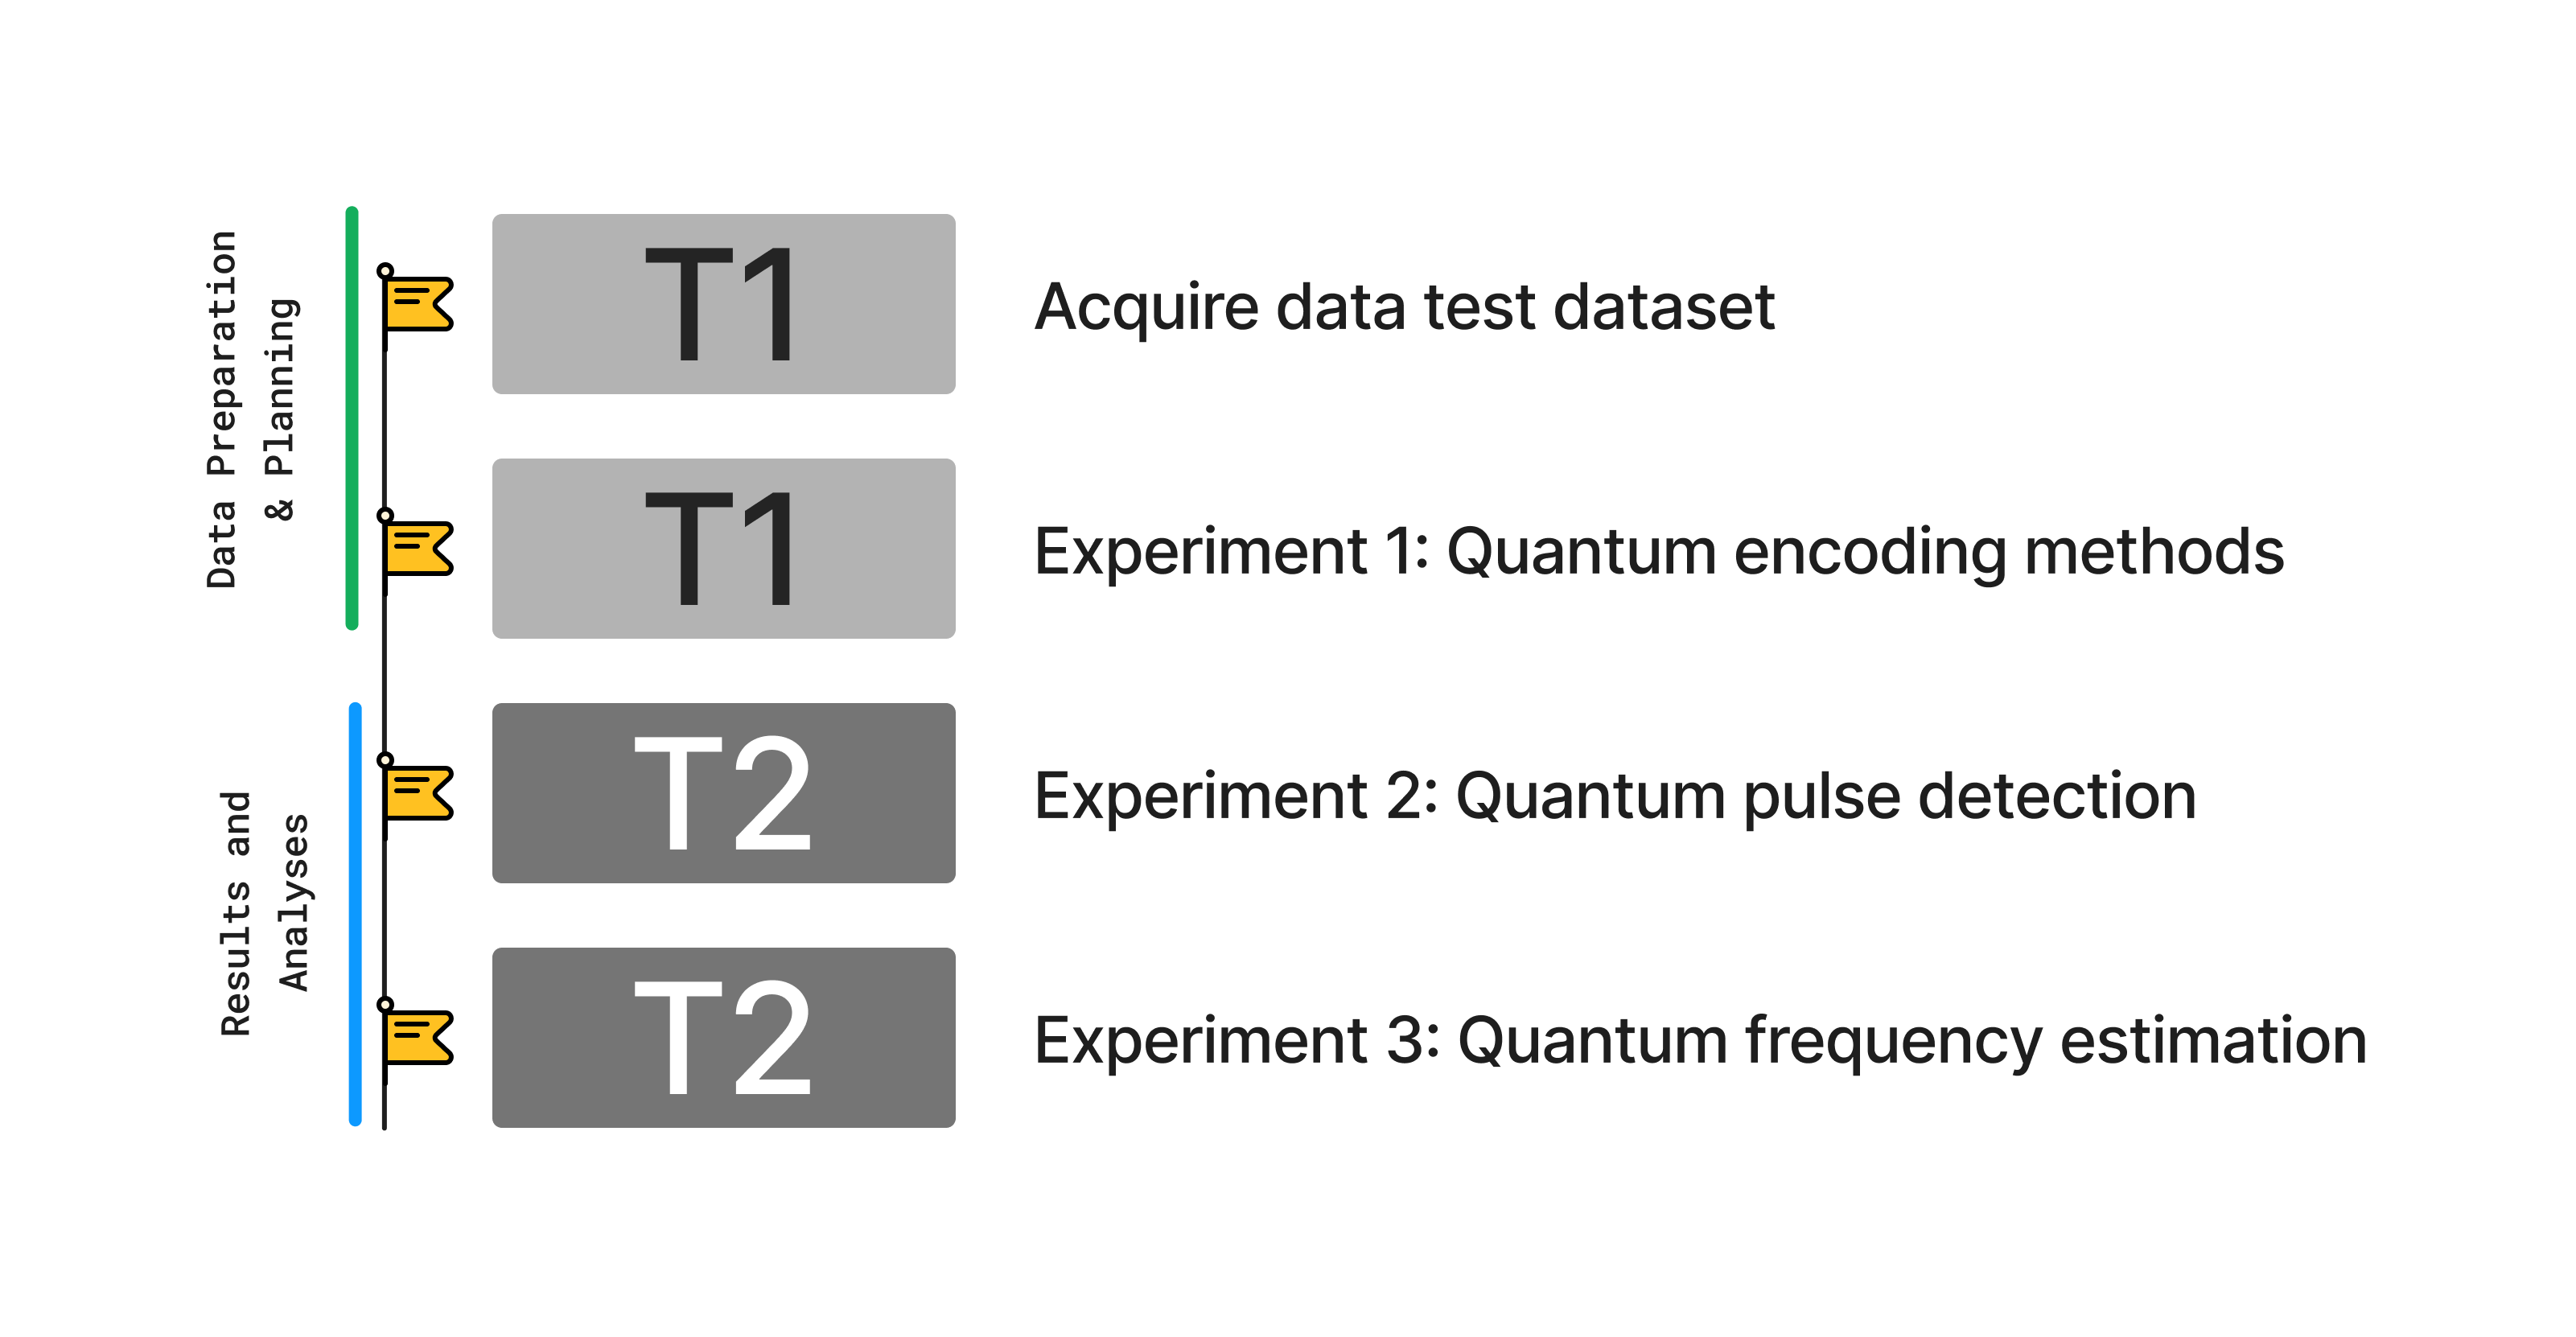
\includegraphics[width=1\textwidth]{Figures/roadmap.png}
    \caption{Research roadmap}
    \label{fig:roadmap}
\end{figure}

\section{Artefact Development Approach}~\label{sec:approach}

% ---------------- EXPERIMENT 1 ---------------- %

\subsection{Experiment 1: Data encoding}
\todo{I can't figure out how to just number these paragraphs as experiment 1, 1.1, etc. I've put them like this for now...}
% How encoding influences the next experiments.
\todo{need to make clear that the experiments are independent, but influenced by the learnings of the previous. Discussion will cover exactly \textbf{what} was taken / influenced (Flexible research design)}
Firstly, before any quantum signal processing may be conducted, signals must be encoded into qubits from the classical source data.
Encoding is a necessary prerequisite for any subsequent quantum processing to be conducted, and therefore will be the object of the first experiment.

%%% Design
Using a combination of classical signal processing techniques to prepare data, and known quantum methods, the first experiment aims to encode classical signals into qubits.
% Statement of the problem

The incident signal prior to sampling is a continuous complex-valued function
$x : \mathbb{R} \rightarrow \mathbb{C}, t \mapsto x(t)$,
where $x(t)$ represents the complex amplitude of the signal at any given time, $t \in \mathbb{R} > 0$.

After being sampled, the signal is discrete.
$x : \mathbb{N} \rightarrow \mathbb{C}, t \mapsto x[t]$,
where $x[n] = x(n T_s)$, the $n^{th}$ sample of the signal, $n$ is an integer representing the sample index, and $T_s$ is the sampling period (i.e., $T_s = 1/f_s$).

Let $\mathbf{x}$ be the buffer of samples $x_n=x[n]$.

The goal of this encoding is to prepare the sample buffer for quantum processing.
Several methods will be implemented and evaluated.

\textbf{Basis encoding}

\todo{Still revising the particulars here... (also a WIP as I'm missing some encoding methods)}

The simplest of all non-trivial quantum encoding methods, basis encoding, maps a binary string $x \in {\{0,1\}}^n$ as coefficients of basis states.

Let $\vert b_n \rangle$ be the $n^{th}$ orthonormal basis for a $N$-dimensional quantum system.
Then any state of the system can be written as a linear combination of the basis states:
\begin{equation}
    \displaystyle{
        \phi: \mathbb{R}^n \rightarrow | \mathbf{x} \rangle =
        \sum_{i=0}^{N}
            c_i | b_i \rangle
    }
\end{equation}
Where $c_i$ are complex coefficients of the basis states which satisfy the normalisation condition
\begin{equation}
    \displaystyle{\sum_{i=1}^n |c_i|^2 = 1}
\end{equation}

For example, encoding $\mathbf{x} = (1, -1+i\sqrt{3}, 1, 1+i\sqrt{3})$

The normalisation condition must be be upheld. 
One way to ensure this is to divide each element of the vector by the Euclidean norm.
\begin{equation}
    \displaystyle{\mathbf{x} = \frac{1}{\sqrt{6}}(1, -1+i\sqrt{3}, 1, 1+i\sqrt{3})}
\end{equation}
Encoding this into a 2-qubit system implies multiplying each element by the basis states: $|00\rangle, |01\rangle, |10\rangle, |11\rangle$.
Therefore, 
\begin{equation}
    \displaystyle{
        | \mathbf{x} \rangle =
        \frac{1}{\sqrt{6}}
        (
            |00\rangle +
            (-1 + i\sqrt{3}) |01\rangle +
            |10\rangle +
            (1 + i\sqrt{3}) |11\rangle
        )
    }
\end{equation}


\textbf{Amplitude encoding}

Quantum amplitude encoding represents classical information as amplitudes of quantum states.
For $n$ qubits, encoding a classical vector $x \in \mathbb{C}^{n}$ into a quantum state $\vert x \rangle$ is described by:

$|x\rangle = \frac{1}{\sqrt{N}} \sum{_n^N}  x_n \vert y \rangle$


% The operation of encoding is one which maps to a Hilbert space, $\mathcal{H}$.
We can define a map $\phi: \mathbb{R}^n \rightarrow \mathcal{H}$ that takes a vector of length $n$ (i.e., the length of the buffer) and maps it to a vector in the Hilbert space, $\mathcal{H}$.
% The goal of any quantum encoder is to satisfy:
One common choice for $\phi$ is to use the Fourier transform to map the buffer into a frequency representation, and then use the resulting frequency coefficients as the coordinates in $\mathcal{H}$. This can be expressed mathematically as:
\begin{equation}
\phi(x) = \sum_{k=0}^{n-1} x_k e^{i2\pi k t / n}
\end{equation}
This represents the summation of the product of each sample $x_k$ with a complex exponential term $e^{i2\pi k t / n}$, where $t$ ranges from 0 to $n-1$ and $k$ ranges from 0 to $n-1$.


% Criticality of data vs data format.
It should be noted that the specific input parameters of the encoding dataset are not critical, rather it is the format that is a controlled variable.
Given the data themselves have the same qualities of a complex value varying over time, their specific implementation is of lesser importance.
% Types of input data.
In this respect, one \todo{define in literature review}\todo{create appendix with block diagrams of these radars}\textbf{pulse radar} and one \textbf{pulsed-Doppler radar} will be employed as test inputs, as they depict a minimally representative sample of a multi-radar environment. 

%%% Criteria
Specifically, the independent variable is the type of quantum algorithm for encoding time-series signals, and measured will be the sampling capacity, bandwidth, computational efficiency, and expressivity.
%%% Measures
\begin{itemize}
    \item Sampling capacity, defined as the number of samples which can be encoded simultaneously, will be measured the number of samples that can be practically encoded as qubits.
    \item Bandwidth will be measured by the span of frequencies that can be encoded.
    \item Computational efficiency will be recorded as the number of \todo{define in literature review}\textbf{logical qubits and ancillary qubits} required to encode the data.
    \item Expressivity, is "a circuit’s ability to generate (pure) states that are well representative of the Hilbert space" \cite{sim_expressibility_2019} \todo{I'm not sure whether to include this metric...}
    \todo{I don't think these are particularly validated measures. But, I'm not sure if they exist... to confirm...}
\end{itemize}
Since encoding methods produce quantum data that differ in construction, it is important that the structure of quantum data is compatible with the analysis.
The encoded form is more critical than performance and is considered when choosing the encoding method for the following experiments.

% ---------------- EXPERIMENT 2 ---------------- %

\subsection{Experiment 2: Signal detection}

\todo{Diagram of signal with pulse boundary markings. Should have overlapping signals}
% Motivation
After sample data are encoded into qubits, the next challenge is to detect pulse boundaries. This is termed \textit{pulse detection}.
Pulse detection is required in order to understand where pulses exist in time, so as to enable further characterisation of the nature of the transmitted signal.
This technique is only applicable to pulsed radars as they exhibit pulse boundaries; \ac{CW} radar and others of similar nature do not.
It is for this reason, that only pulsed radars will be trialed, with the number independently varying from $1$ to $10$, each with \ac{PW} controlled at $10 \mu s$.
Both pulsed-Doppler and pulsed radar types will be trialed, being a secondary independent variable.
The centre frequency of each radar is to be randomly spread uniformly over the frequency spectrum.
For the pulsed-Doppler trial, the frequency deviation will be controlled at $1MHz$

The technique ultimately developed is not limited to a specific encoding technique, nor is it wholly required that processing be completed in the quantum domain - minimal pre- and post-processing may be applied.
The dependent variable will be a continuous determination of pulse boundaries.
A measured pulse boundary here is defined as the quantitative probability of a pulse rising or falling at any given time.\todo{this is equivilent to TOA/TOE. Possibly re-phrase for clarity}
It should be the result of quantum measurement.

From these raw measurements, the analysis of accuracy may follow, utilising:
\begin{itemize}
    \item precision metric:
- \todo{Continuous version of??} P/(TP+TN)
    \item Recall metric:
- \todo{Continuous version of??} P(TP/FN)
    \item F1 score:
- \todo{Continuous version of??} 2*(precision+recall) / (precision*recall)
\end{itemize}

% ---------------- EXPERIMENT 3 ---------------- %

\subsection{Experiment 3: Frequency Estimation}

%%% Design
% Description
Finally is the experiment testing the performance of a quantum frequency estimation algorithm.
% Purpose / criteria
The algorithm's goal is to output a frequency indication given some encoded signal input.
% Types of input data.
Not included in the scope of this experiment is dealing with non-constant signal envelopes; that is, continuous waves are only to be examined.
Consequently, only a single \ac{FMCW} or \ac{CW} radar types will be simulated in independent trials.
Also varied will be the independent variable \ac{SNR} ranging from $0dBC$ (no noise), to $70dBC$.
% Nature of solution
Again there is no prescriptive specific encoding technique, nor is it limited to solely quantum
methods.
\todo{define the frequency modulation rate and type.}
The quantum method should output a most probable frequency indication for each quantised sample.
%%% Measures
The measure of accuracy will be a \ac{RMSE} frequency error, aggregated over all samples. \todo{I'm not sure how this stacks up with many samples. Does \ac{RMSE} accumulate?}

% --------------
%%% Qualitative stuff / post hoc evals
% For although subsequent experimental trials and post hoc evaluation of the encoding methods remain as important means of assessing its suitability to the broader question, each experiment is designed to be independent of the results of the previous.
% In other words, while the success of the subsequent analyses hinges only somewhat on the quantitative comparison of encoding methods, it is the understanding of <...>. 
% Is is empirical trial and post hoc evaluation that measure this. 

% The method consists of creating a GNU-Radio block that permits the input of complex-valued samples into a buffer. The processing of samples is then done in Python and Qiskit within that block, and finally, outputted to a buffer where it is recorded.
-----------------------

To achieve the objective of \textbf{acquiring radar signal test data}, \todojc{Free and open access emulator / generator perhaps, is your preference not the necessity, may be skip "free and open access" your solution could secure such a device. 
Also another approach still is to acquire some data set, which you may need to acknowledge here.}\textbf{a free and open-access signal emulator} will need to be acquired and validated. 
It should have capability of  generating a set of radar signals exhibiting various degrees of signal quality and environmental situations. 
The variable signal quality refers to a signal-to-noise ratio, and environmental conditions refer to number of radars, pulse density, and pulse frequency.






% It may also be suggested that a frequency-domain input space be explored, in which case, the same experimental methodology should be applied, substituting IQ for a time varying frequency input. The reason for proposing a frequency-domain input signal is due to the general bandwidth limitation of practical IQ measurements as well as the more representative nature of frequency plots for radar signals.

% % Quantum analysis algorithms:

% The stages in the of development the artefact are:
% \begin{quote}
%     \textit{
%         \begin{enumerate}
%             \item Encode the input data into the state of a set of qubits.
%             \item Bring the qubits into superposition over many states (i.e., use quantum superposition).
%             \item Apply an algorithm (or oracle) simultaneously to all the states (i.e., use quantum entanglement amongst the qubits); at the end of this step, one of these states holds the correct answer.
%             \item Amplify the probability of measuring the correct state (i.e., use quantum interference).
%             \item Measure one or more qubits.
%         \end{enumerate}
%         - Quantum computing for finance: Overview and prospects: Román Orús, Samuel Mugeld, Enrique Lizaso \todo{Add this to citations}
%     }
% \end{quote}

% \subsection{Frequency estimation}

% instead of descretising signals into definite PDW's, the Quantum system might be able to generate a superposition of all possibilities of potential signal parameters at once. Further processing such as pulse detection and de-interleaving may be able to be conducted at once. This approach would investigate whether quantum methods can be used to place observed radar modes into a super-positioned and continuous state.
\section{Empirical Evaluation}~\label{sec:evaluation}


\subsection{??Research Questions (RQs)??}~\label{subsec:RQs}
\section{Results \& Discussion}~\label{sec:discussion}

\section{Threats to Validity}~\label{sec:threats}

\subsection{Project Risks}

\subsubsection{Technical limitations}

\textbf{Risk}

Quantum computing technologies are new and undeveloped, with practical implementations potentially unsuitable or impossible given the current state of the technology. These limitations may hinder achieving of the research objectives.

\textbf{Mitigation}

If this limitation is affronted, either reduce scope, or trial alternative approaches.
% 
\subsubsection{Data quality}

\textbf{Risk}

The quality of the data may be insufficient: as the acquisition of real data was deemed impractical, generated data were used and as a result of limited time and scope, it may be non-representative or inadequate for achieving all research objectives. 

\textbf{Mitigation}

Improve the radar data models and validate it with additional data sources to ensure a representative dataset. 
% 
\subsubsection{Time constraints}

\textbf{Risk}

Since the honours thesis is inherently time constrained, the project timeline and deadlines may prove insufficient to thoroughly explore and answer all research questions.
Furthermore, inadequate time management could result in rushed or incomplete work-products, and thereby potentially compromise the quality of the research.

\textbf{Mitigation}

Create a detailed project plan with definite milestones and deadlines. Seek guidance from supervisor to ensure time management and focus are maintained.
% 
\subsubsection{Scope creep}

\textbf{Risk}

The research project may face the risk of scope creep, wherein additional objectives, or analysis – outside of scope - are added. This may lead to a loss of methodological rigor and risk of not achieving the defined research objectives.

\textbf{Mitigation}

Define the research scope and objectives clearly from the beginning. If a scope change is required, seek advice from supervisor and produce a written deviation justification.
% 
\subsubsection{Ethical considerations}

\textbf{Risk}

While no serious ethical concerns were raised, there is a small risk that this research could be deemed sensitive, which risks any future dissemination plans.

\textbf{Mitigation}

Review security assessments and maintain transparent documentation throughout the process.
% 
\subsubsection{Resource limitations}

\textbf{Risk}

Due to this research requiring access to cloud-hosted quantum computers, a lack of funding for this service may impact the ability to achieve the research objectives.

\textbf{Mitigation}
Seek whether physical hardware is required, and if so, optimise resource usage by prioritising critical experiments. Cost limitations could be mitigated by seeking funding from the university.

\section{Conclusion \& Future Work}~\label{sec:conclusion}
\subsection{Future Work}~\label{subsec:future}


%-------- Bibliography
\newpage
\singlespacing
% \bibliography{references} %%All bibtex references are in references.bib file
% \bibliographystyle{siam}
\bibliographystyle{ieeetr}
% \bibliographystyle{jcabbrv} % Sorted and "note" fields removed
% Auto-imported from Mark's Zotero
\bibliography{zotero_references.bib}
% Manual imports
% \bibliography{references.bib}
\end{document}
%-------------DOCUMENT END-------------------